\documentclass[11pt]{article}

\usepackage[margin=1in]{geometry}
\usepackage{graphicx}
\usepackage{caption}
\usepackage{subcaption}
\usepackage{booktabs}
\usepackage{hyperref}

\title{A Simple Workflow for Processing and Visualizing Experimental Data}
\author{The Author}
\date{February 22, 2026}

\begin{document}
\maketitle

\begin{abstract}
This short article demonstrates a minimal data workflow for reading raw data,
applying basic processing steps, and generating figures for reporting. The
pipeline is intentionally lightweight and serves as a template for
reproducible analysis and visualization.
\end{abstract}

\section{Introduction}
Scientific results often rely on repeatable transformations from raw
measurements to processed signals and summary figures
\cite{wilkinson2016fair,lowe2019good}. This demo project shows an end-to-end
workflow that reads tabular data, applies smoothing and derivative
calculations, and produces publication-ready plots
\cite{tufte2001visual}.

\section{Methods}
Raw data are read from \texttt{data/raw.csv}. The processing script performs
the following steps:
\begin{itemize}
  \item drops rows with missing values,
  \item detects a time column when available (or uses row index),
  \item computes a moving-average smooth for numeric columns, and
  \item computes time derivatives for numeric columns.
\end{itemize}
Processed data are written to \texttt{data/processed.csv}. The visualization
script creates time-series and distribution plots for both raw and processed
data, as well as plots for smoothed signals and derivatives when available
\cite{mckenna2021dataviz}.

\section{Results}
Figure~\ref{fig:raw} shows raw time-series and distributions.
Figure~\ref{fig:advanced} shows advanced visualizations.
Figure~\ref{fig:processed} shows processed time-series, smoothed signals, and
time derivatives.

\begin{figure}[ht]
  \centering
  \begin{subfigure}[t]{0.48\textwidth}
    \centering
    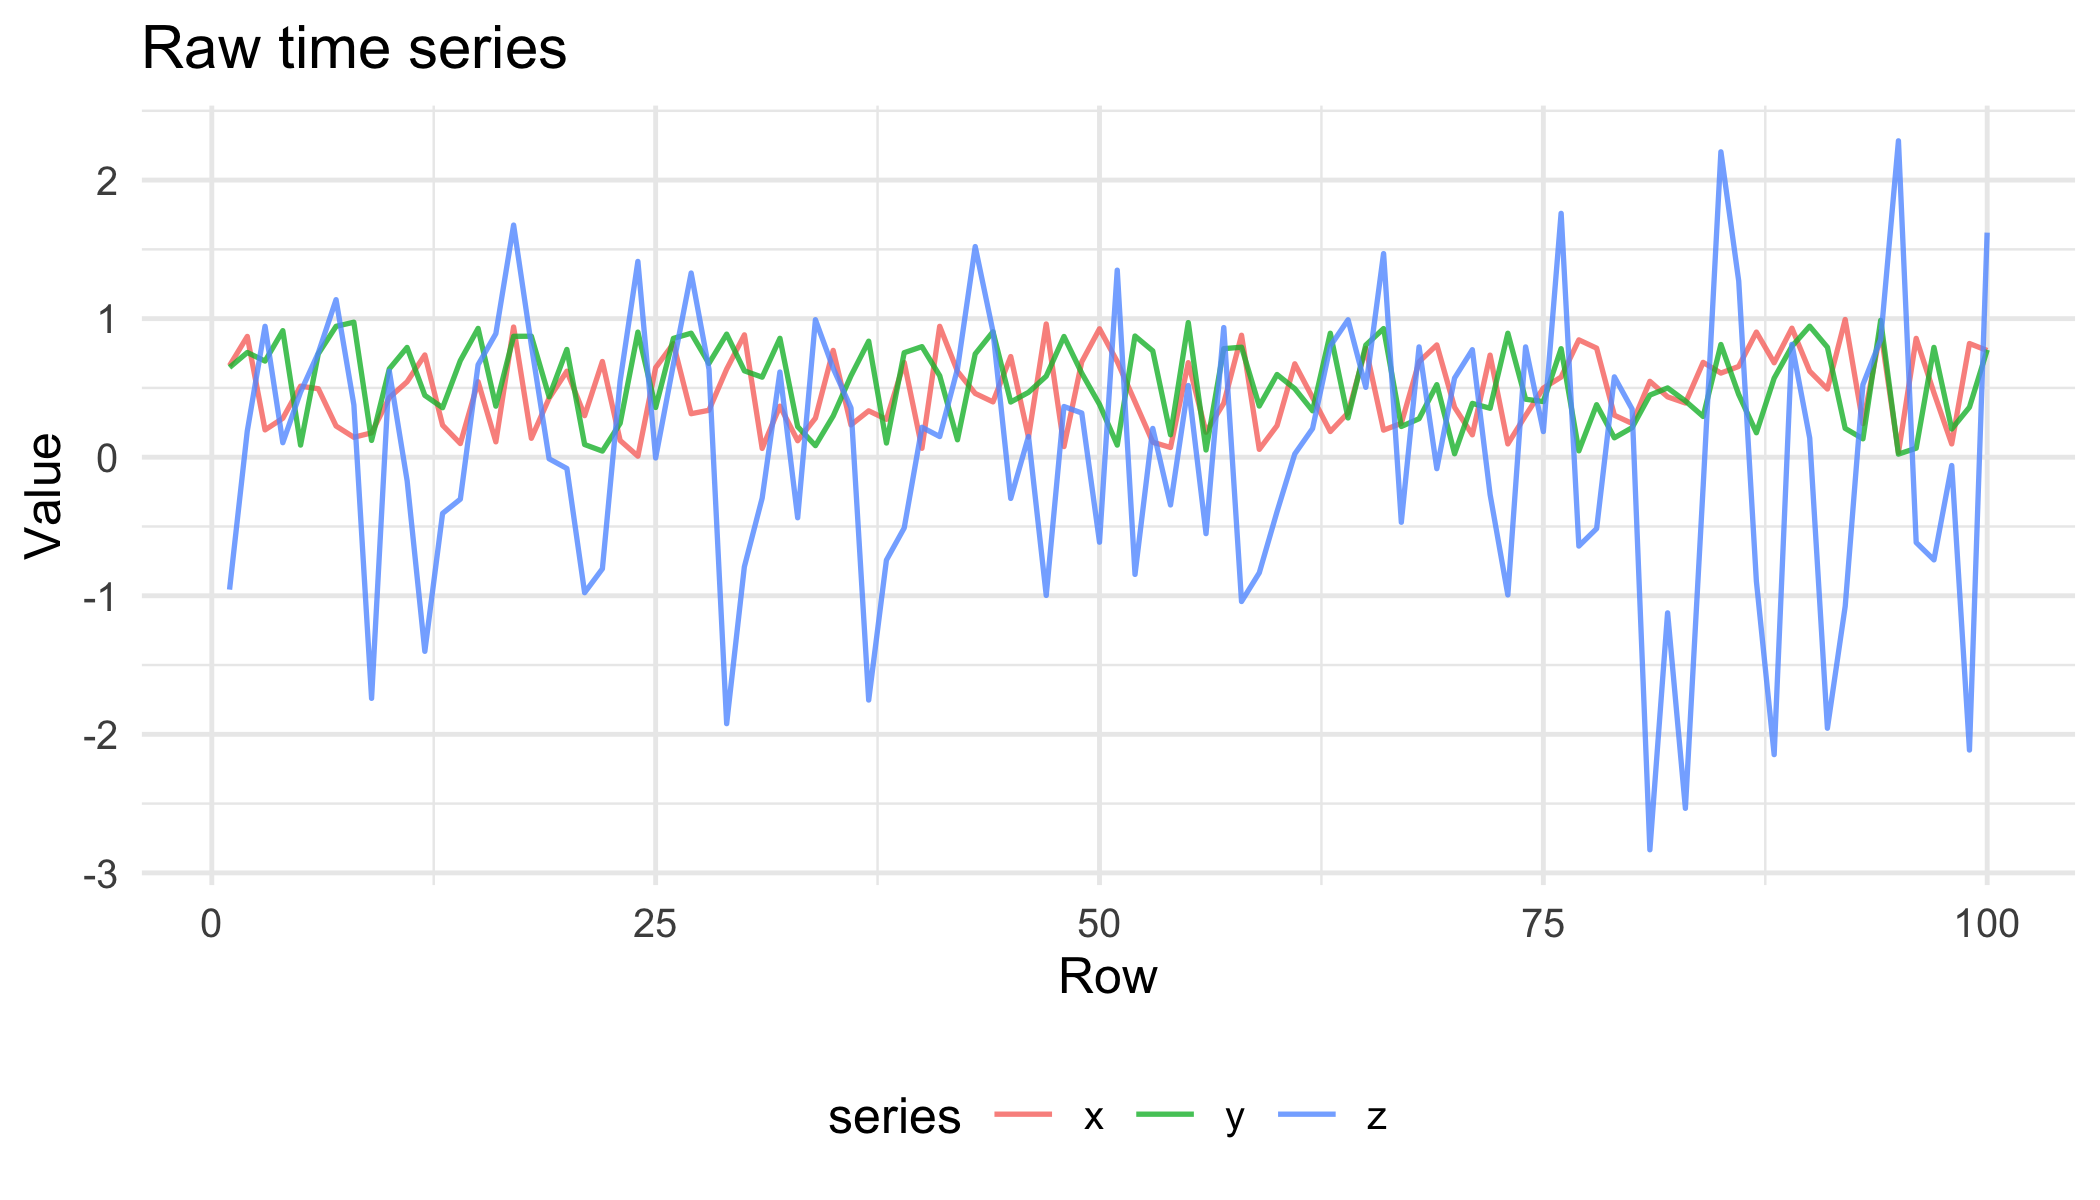
\includegraphics[width=\textwidth]{figures/raw_timeseries.png}
    \caption{Raw time series.}
  \end{subfigure}
  \hfill
  \begin{subfigure}[t]{0.48\textwidth}
    \centering
    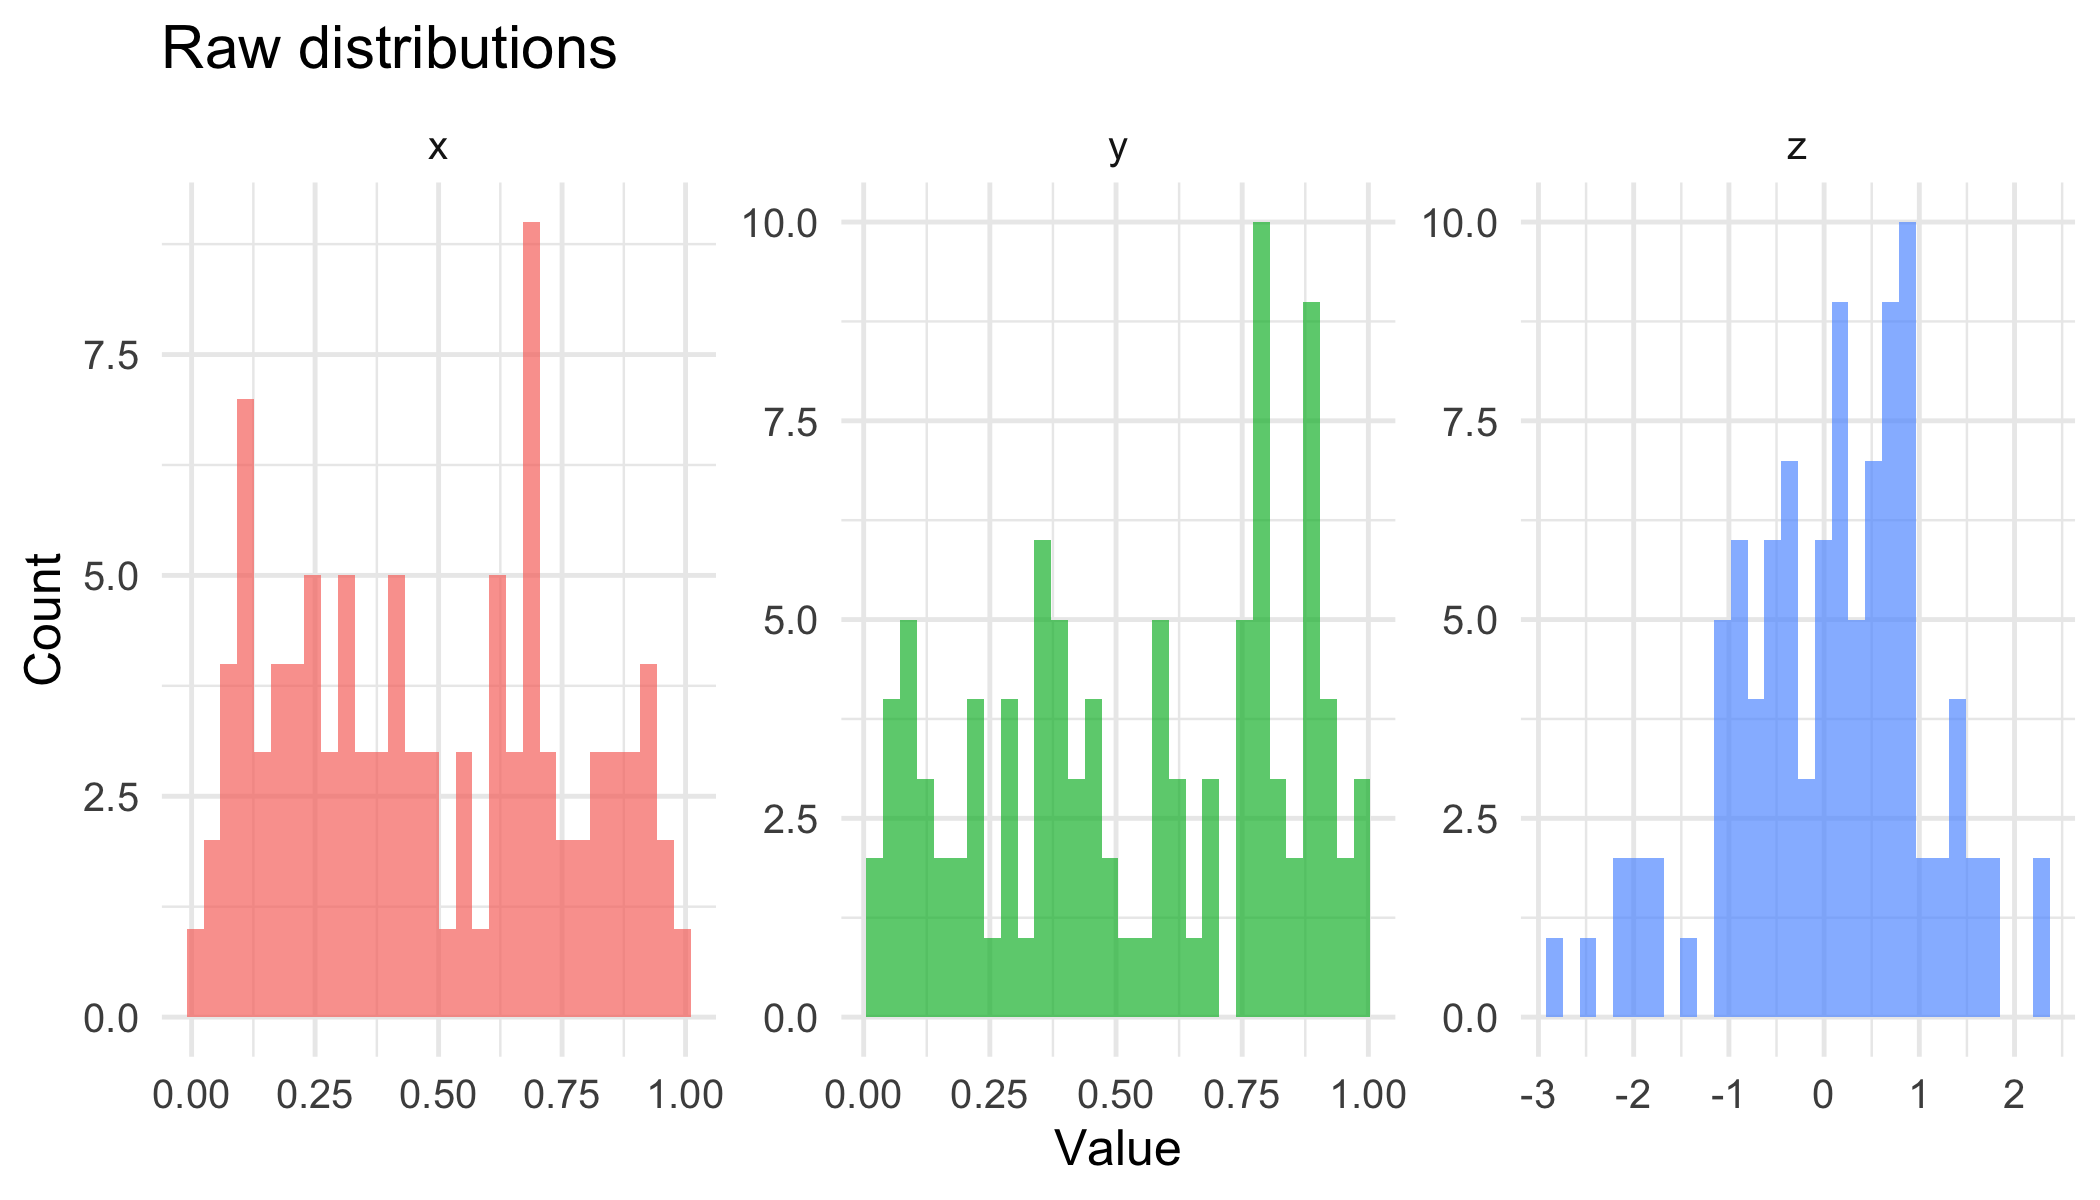
\includegraphics[width=\textwidth]{figures/raw_distributions.png}
    \caption{Raw distributions.}
  \end{subfigure}
  \caption{Raw data visualizations.}
  \label{fig:raw}
\end{figure}

\begin{figure}[ht]
  \centering
  \begin{subfigure}[t]{0.48\textwidth}
    \centering
    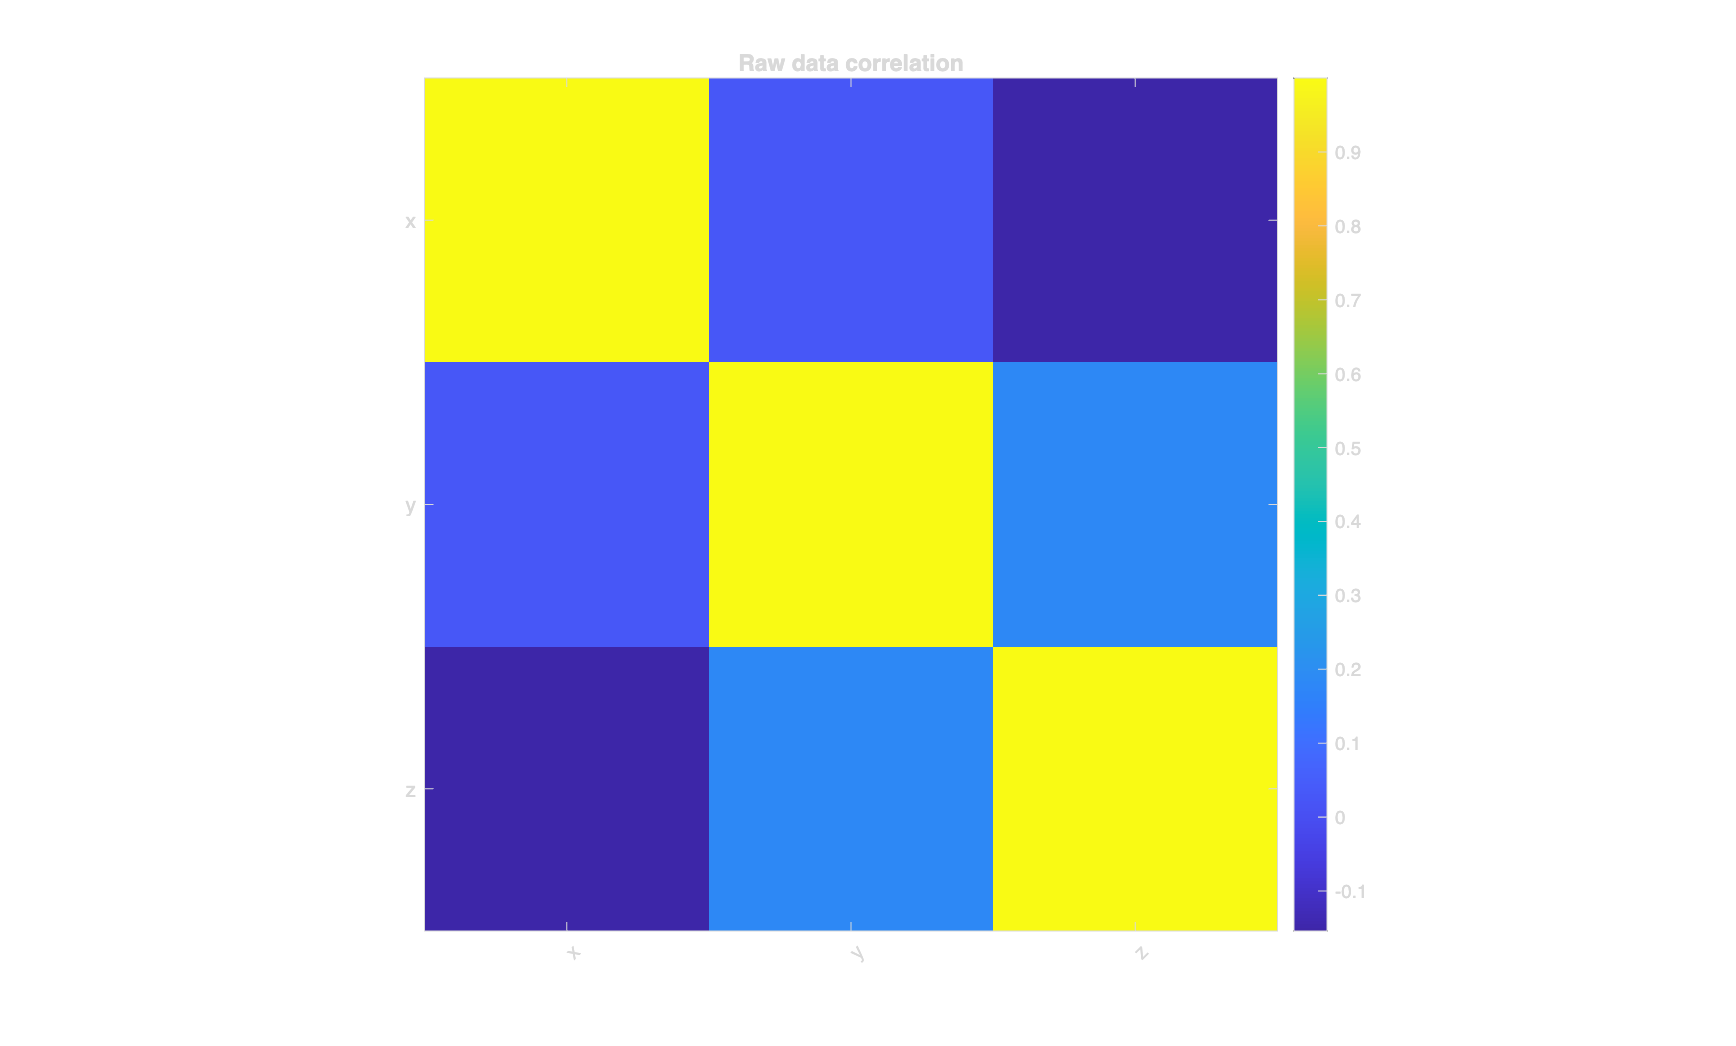
\includegraphics[width=\textwidth]{figures/raw_correlation.png}
    \caption{Correlation heatmap.}
  \end{subfigure}
  \hfill
  \begin{subfigure}[t]{0.48\textwidth}
    \centering
    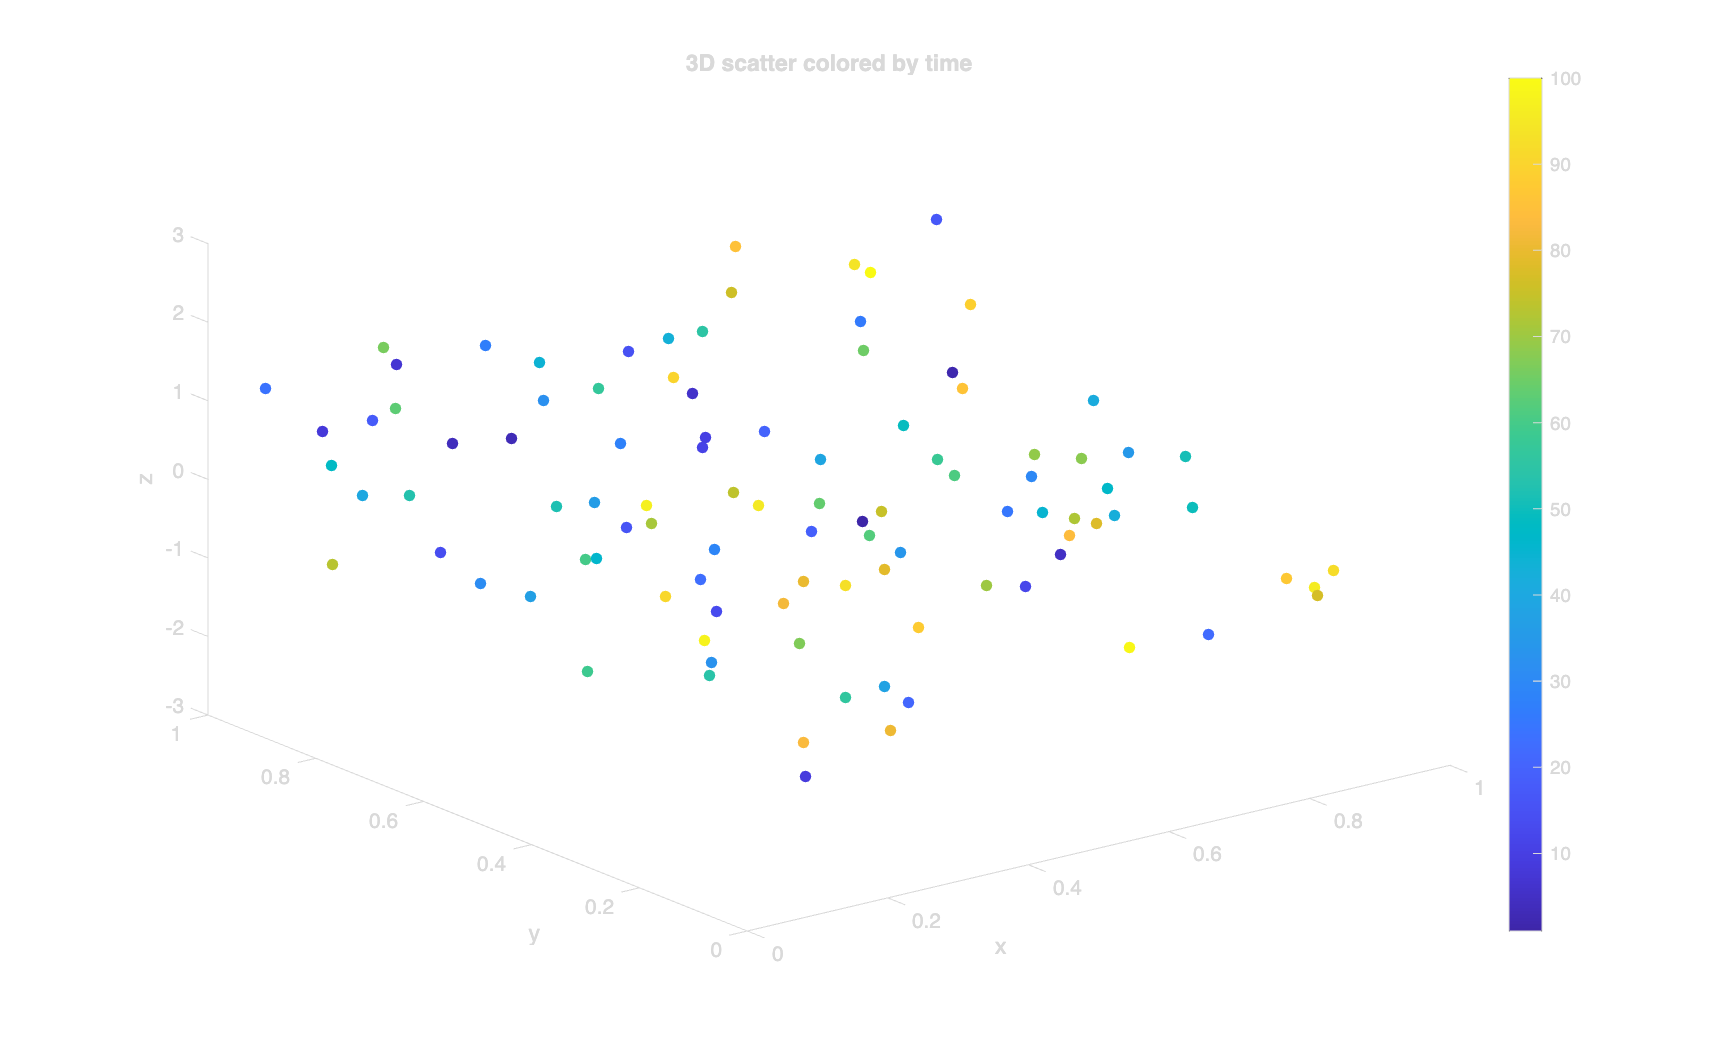
\includegraphics[width=\textwidth]{figures/raw_scatter3d.png}
    \caption{3D scatter plot colored by time.}
  \end{subfigure}

  \vspace{0.5em}

  \begin{subfigure}[t]{0.48\textwidth}
    \centering
    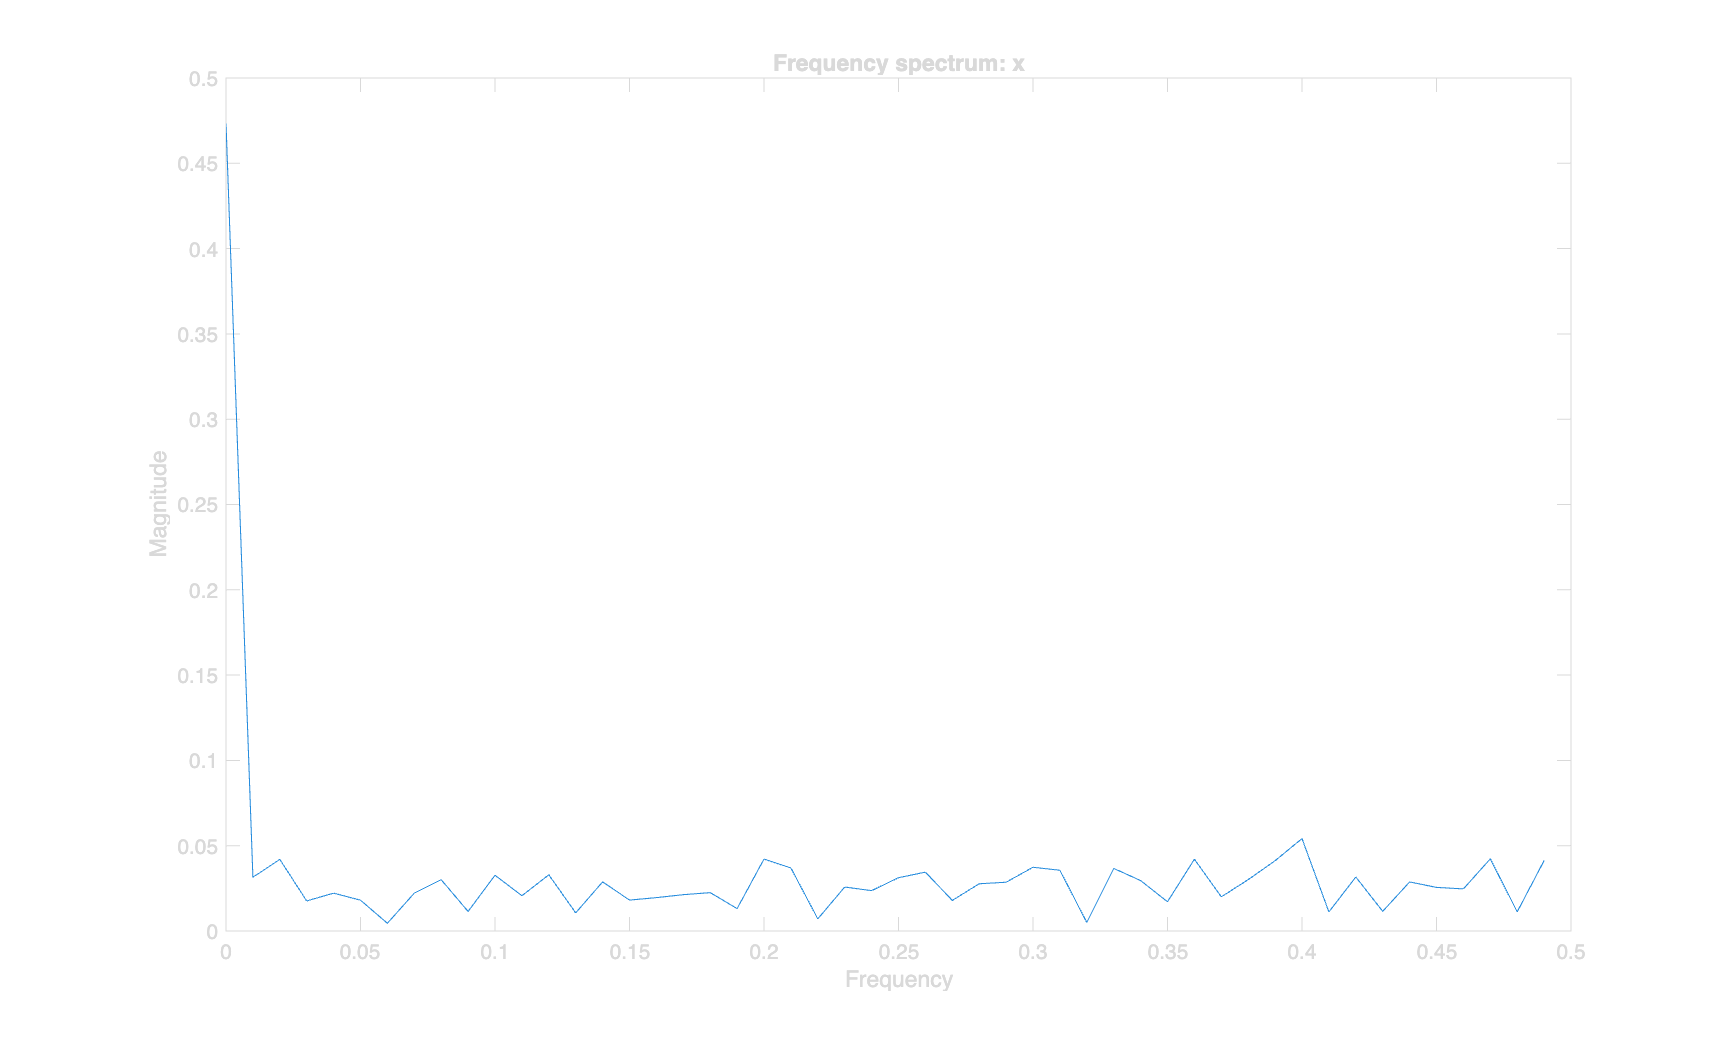
\includegraphics[width=\textwidth]{figures/raw_spectrogram.png}
    \caption{Frequency spectrum.}
  \end{subfigure}
  \hfill
  \begin{subfigure}[t]{0.48\textwidth}
    \centering
    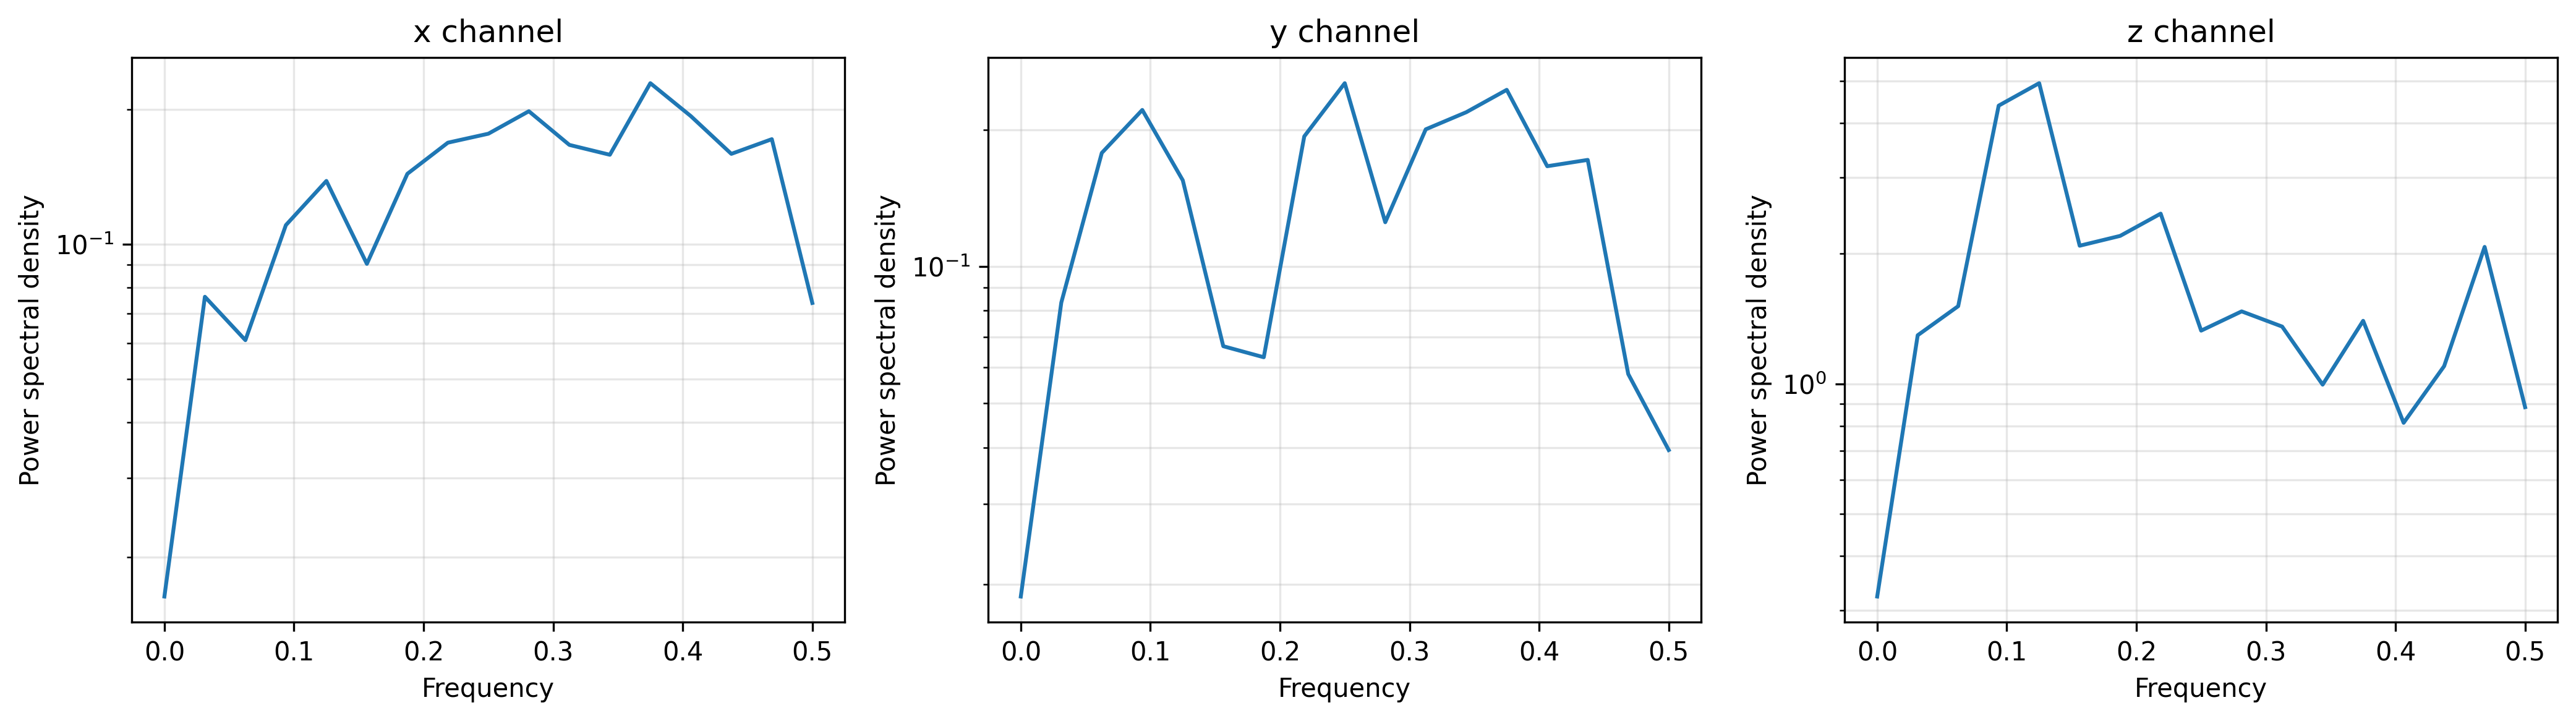
\includegraphics[width=\textwidth]{figures/raw-data-spectra.png}
    \caption{Data spectra.}
  \end{subfigure}
  \caption{Advanced raw data visualizations.}
  \label{fig:advanced}
\end{figure}

\begin{figure}[ht]
  \centering
  \begin{subfigure}[t]{0.48\textwidth}
    \centering
    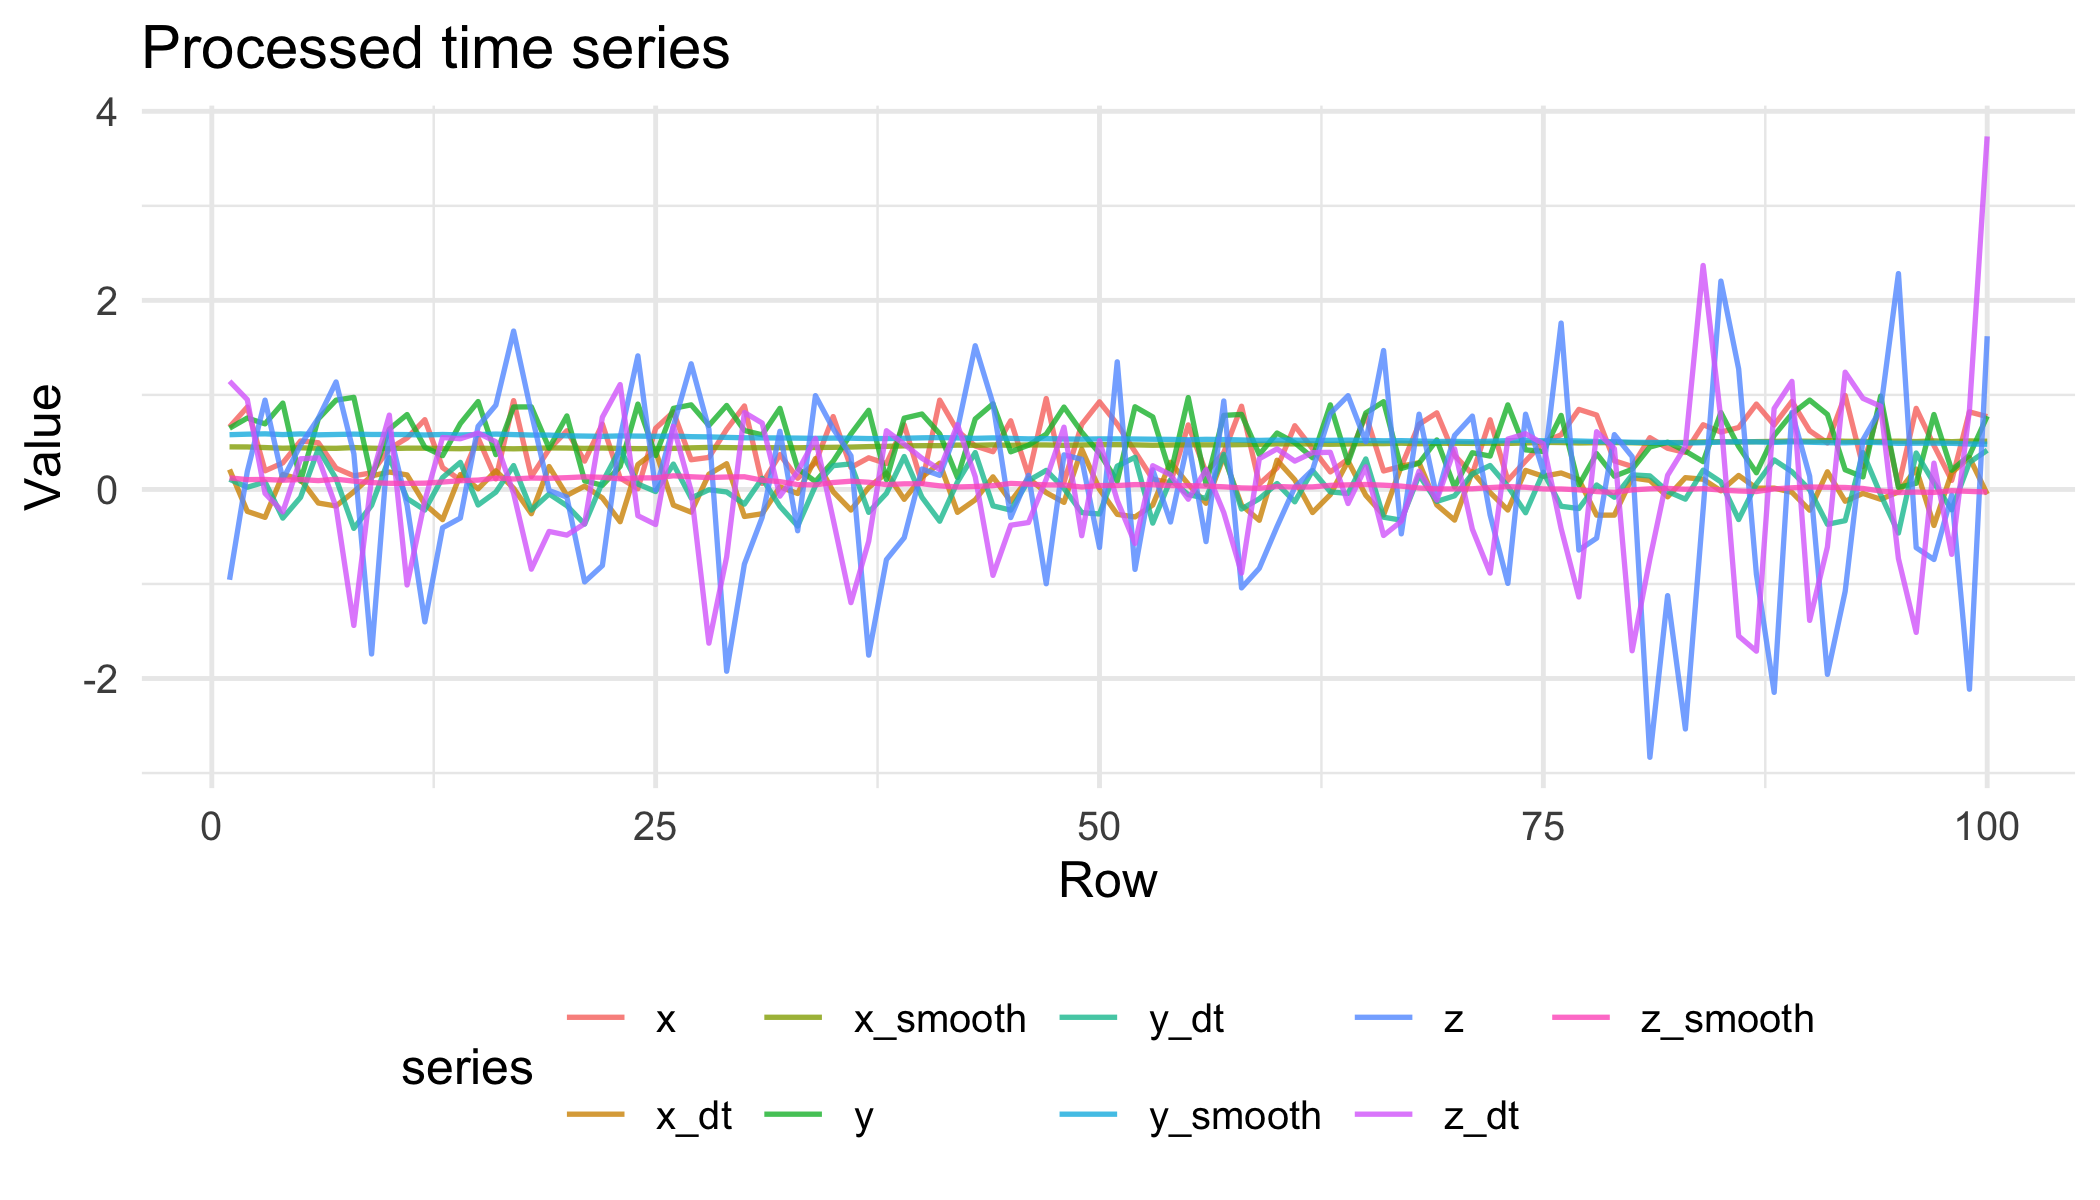
\includegraphics[width=\textwidth]{figures/processed_timeseries.png}
    \caption{Processed time series.}
  \end{subfigure}
  \hfill
  \begin{subfigure}[t]{0.48\textwidth}
    \centering
    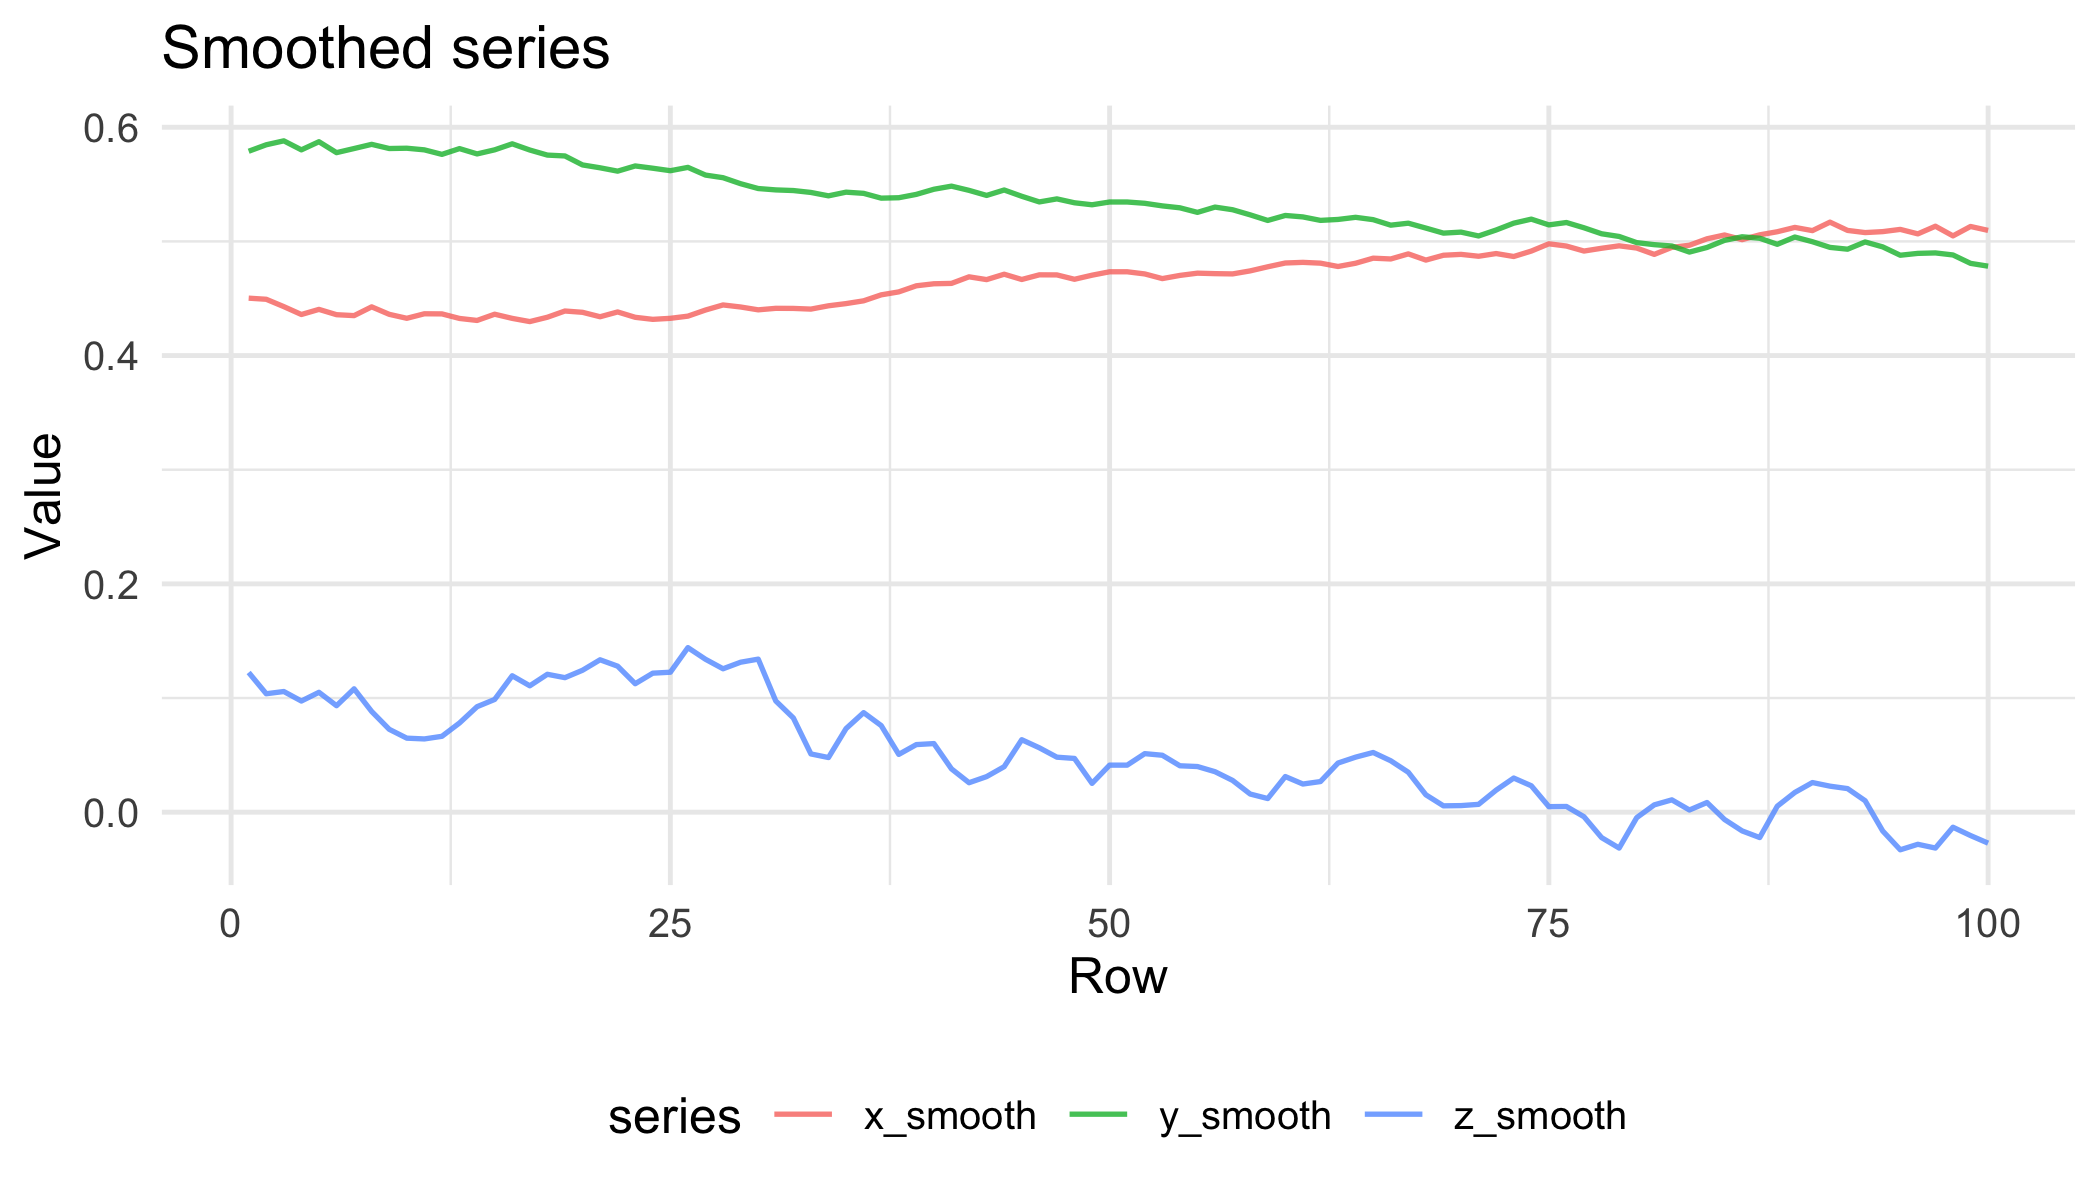
\includegraphics[width=\textwidth]{figures/processed_smooth.png}
    \caption{Smoothed signals.}
  \end{subfigure}

  \vspace{0.5em}

  \begin{subfigure}[t]{0.48\textwidth}
    \centering
    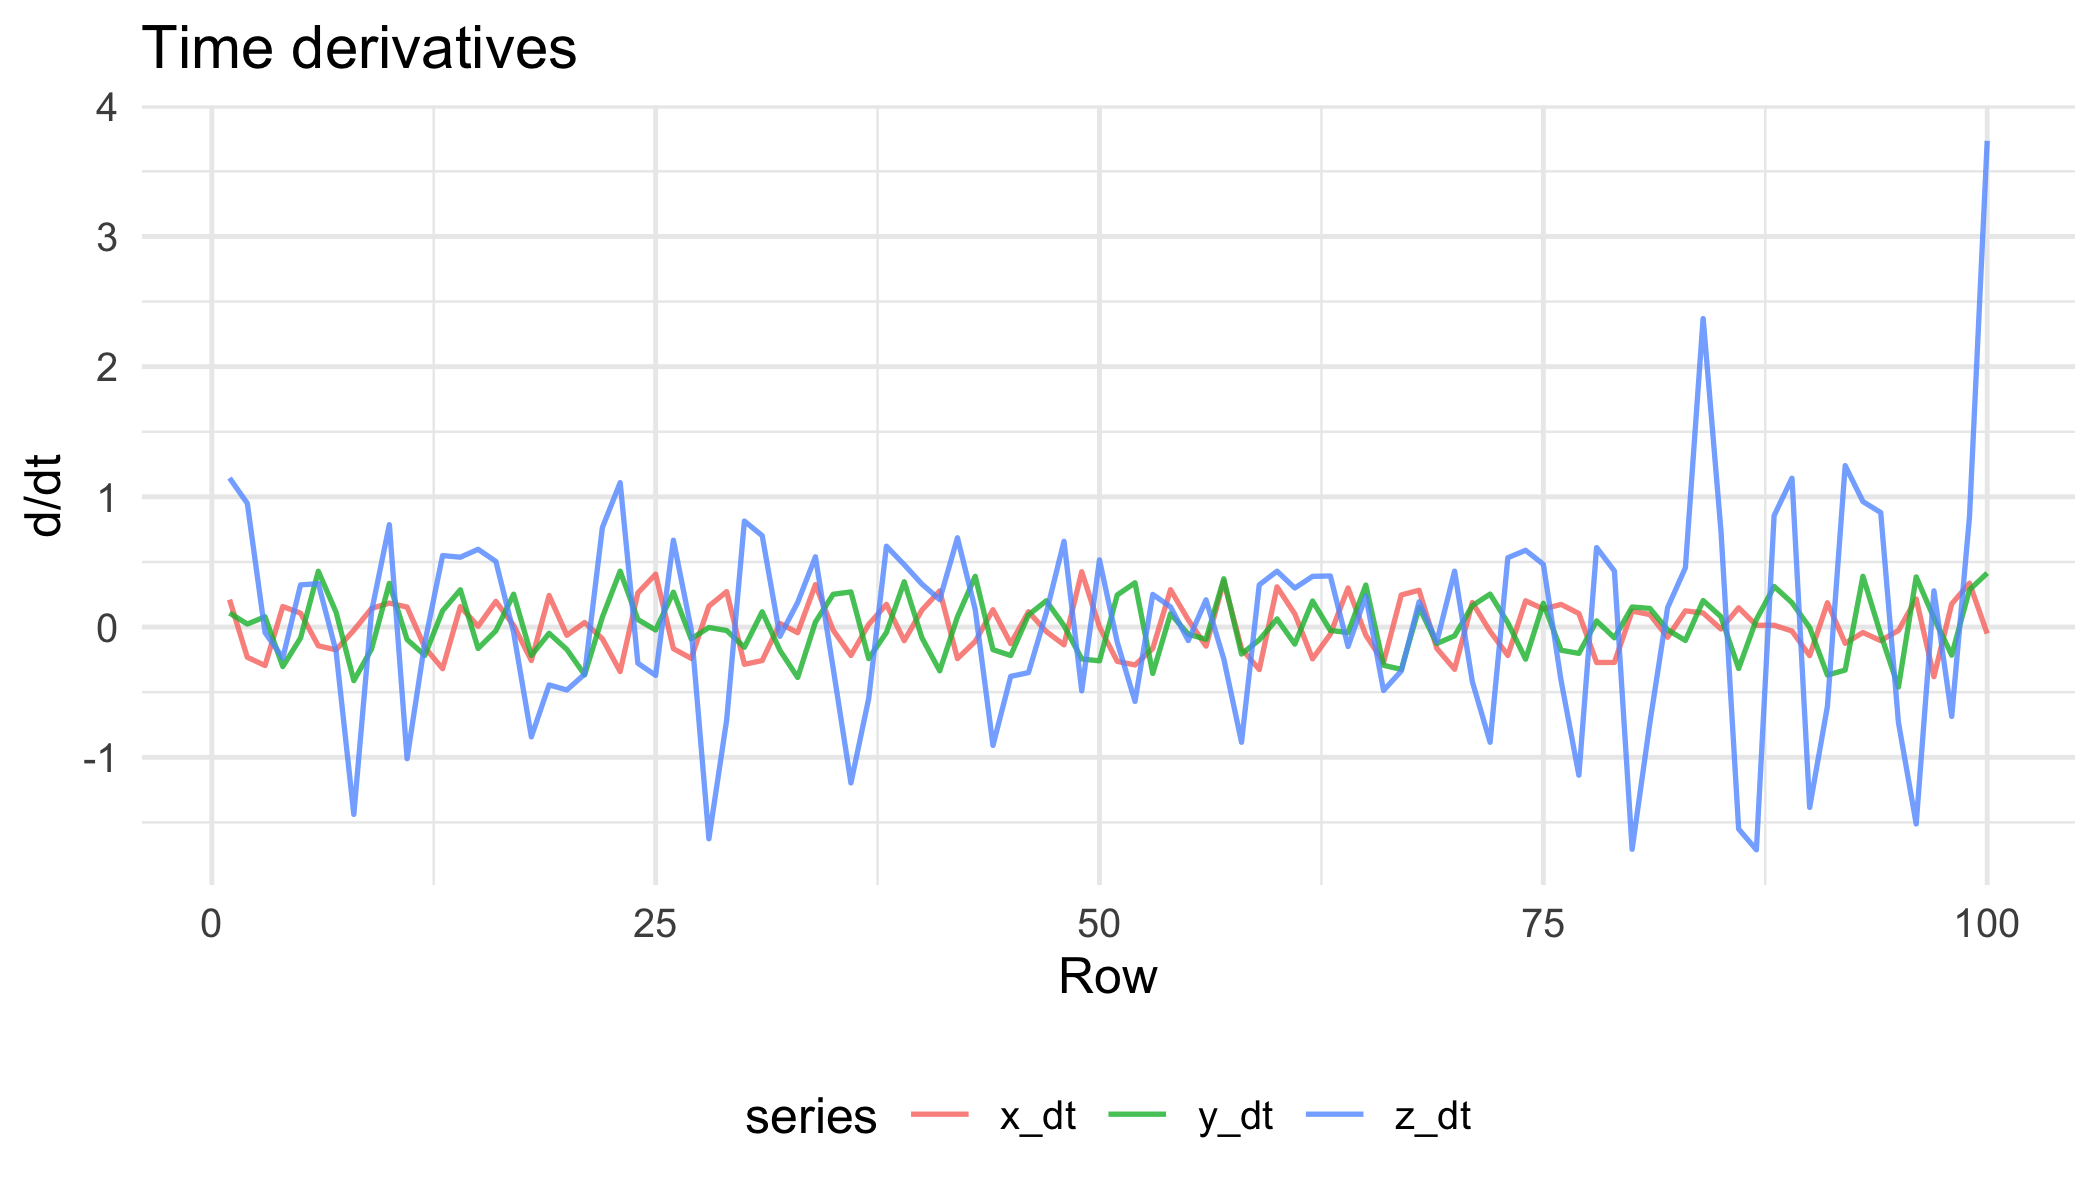
\includegraphics[width=\textwidth]{figures/processed_derivative.png}
    \caption{Time derivatives.}
  \end{subfigure}
  \hfill
  \begin{subfigure}[t]{0.48\textwidth}
    \centering
    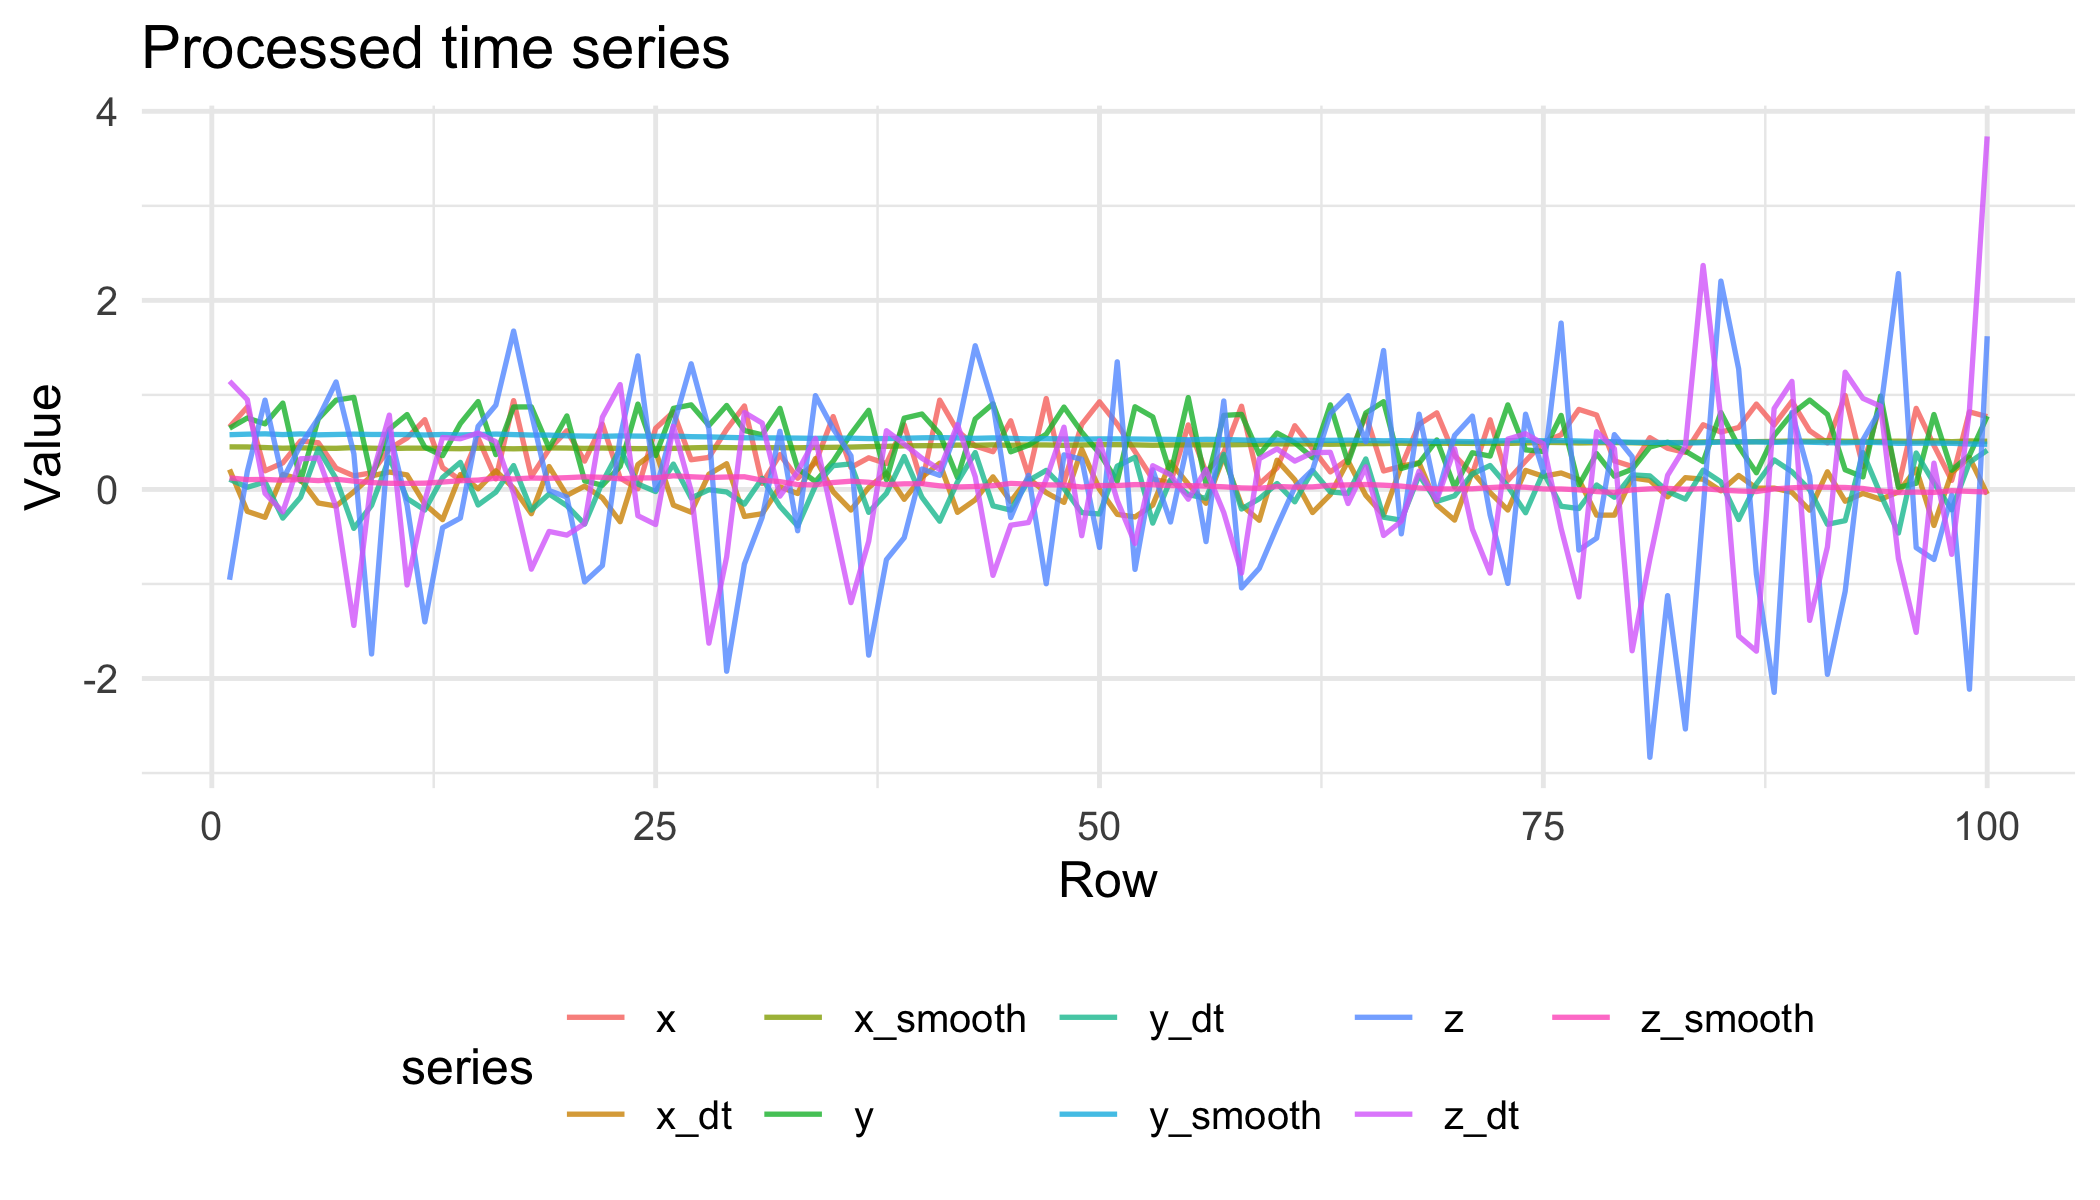
\includegraphics[width=\textwidth]{figures/processed_timeseries.png}
    \caption{Processed overview (repeat for layout balance).}
  \end{subfigure}
  \caption{Processed data visualizations.}
  \label{fig:processed}
\end{figure}

\section{Discussion}
This demo highlights a reproducible workflow that turns raw tabular data into
processed signals and figures suitable for inclusion in a report. The scripts
can be extended with domain-specific processing and more refined
visualization styles.

\section{Conclusion}
The provided scripts and figures form a compact, reproducible analysis
pipeline. They can be adapted for small experiments or larger studies with
minimal modifications.

\bibliographystyle{plain}
\bibliography{references}

\end{document}
